% begin module derivative-sine
\begin{frame}
\begin{align*}
\text{Let}\quad f(x) & = \sin x. \\
\text{Then}\quad f'(x) & =  %
\uncover<2->{%
\lim_{h\rightarrow 0}\frac{f(x+h)-f(x)}{h}%
}%
\uncover<3->{%
 = \lim_{h\rightarrow 0}\frac{\alert<handout:0| 4>{\sin (x+h)}-\sin x}{h}%
}\\%
& \uncover<4->{ = }  %
\uncover<4->{%
\lim_{h\rightarrow 0}\frac{\alert<handout:0| 4>{\sin x \cos h + \cos x \sin h} - \sin x}{h}%
}\\%
& \uncover<5->{ = }  %
\uncover<5->{%
\lim_{h\rightarrow 0}\left[ \frac{\sin x \cos h - \sin x}{h} + \frac{\cos x \sin h}{h}\right] %
}\\%
& \uncover<6->{ = }  %
\uncover<6->{%
\lim_{h\rightarrow 0}\left[ \sin x\left( \frac{\cos h - 1}{h}\right) + \cos x\left( \frac{\sin h}{h}\right) \right] %
}\\%
& \uncover<7->{ = }  %
\uncover<7->{%
\alert<handout:0| 8-9>{\lim_{h\rightarrow 0} \sin x}\cdot \alert<handout:0| 12>{\lim_{h\rightarrow 0} \frac{\cos h - 1}{h}} + \alert<handout:0| 10-11>{\lim_{h\rightarrow 0}\cos x}\cdot \alert<handout:0| 12>{\lim_{h\rightarrow 0}  \frac{\sin h}{h}}  %
}\\%
& \uncover<8->{ = }  %
\uncover<8->{%
\alert<handout:0| 8-9>{\uncover<9->{\sin x}}\cdot \alert<handout:0| 12>{\lim_{h\rightarrow 0} \frac{\cos h - 1}{h}} + \alert<handout:0| 10-11>{\uncover<11->{\cos x}}\cdot \alert<handout:0| 12>{\lim_{h\rightarrow 0}  \frac{\sin h}{h}}  %
}%
\end{align*}
\uncover<12->{%
We need to do more work to find the other two limits.

}%
\end{frame}

\begin{frame}
\begin{columns}[c]
\column{.6\textwidth}
\[
\text{Claim:}\quad \lim_{\theta \rightarrow 0}\frac{\sin \theta }{\theta} = 1
\]
First suppose $0 < \theta < \frac{\pi}{2}$.  Then we can write $\sin \theta$ using ratios of side lengths of a triangle.
\column{.4\textwidth}
\psset{xunit=1.2cm, yunit=1.2cm}
\begin{pspicture}(-0.2, -0.2)(1.2,1.9) 
\psframe*[linecolor=white](-0.2,-0.2)(1.2,1) 
\tiny 
\psline[linecolor=gray!1](3.2, 2)(3.25, 2.05)

\only<1-4, 8->{\psplot[linewidth=0.3pt]{2.598076211}{3}{9 x x mul sub sqrt}
}
\only<5-7>{
\psplot[linecolor=red, linewidth=0.3pt] {2.598076211}{3}{9 x x mul sub sqrt}
}

\psline[linewidth=0.3pt](0,0)(3,0)
\psline[linewidth=0.3pt](0,0)(2.598076211,1.5)
\psline[linewidth=0.3pt](-0.05,0.08660254)(2.548076211,1.58660254)
\psline[linewidth=0.3pt](-0.025, 0.04330127) (-0.075, 0.12990381)
\psline[linewidth=0.3pt](2.573076211, 1.54330127) (2.523076211, 1.62990381)
\rput[b](1.25,0.9){$1$}


\only<1-2, 6-7>{ %line BC
\psline[linewidth=0.3pt](2.598076211,0)(2.598076211,1.5)
\psline[linewidth=0.3pt](2.498076211,0)(2.498076211,0.1)(2.598076211,0.1)
}
\only<3-5>{ % line BC
\psline[linecolor=red, linewidth=0.3pt](2.598076211,0)(2.598076211,1.5)
\psline[linecolor=red, linewidth=0.3pt] (2.498076211,0)(2.498076211,0.1)(2.598076211,0.1)
}
\only<8->{ % line BC
\psline[linecolor=gray, linewidth=0.3pt](2.598076211,0)(2.598076211,1.5)
\psline[linecolor=gray, linewidth=0.3pt] (2.498076211,0)(2.498076211,0.1)(2.598076211,0.1)
}
\only<4-5>{ %line AB
\psline[linecolor=red, linewidth=0.3pt](2.598076211,1.5)(3,0)
}
\only<6-7>{ %line AB
\psline[linewidth=0.3pt](2.598076211,1.5)(3,0)
}
\only<8->{ %line AB
\psline[linecolor=gray, linewidth=0.3pt] (2.598076211,1.5)(3,0)
}
\only<10-11>{ % line BD
\psline[linewidth=0.3pt, linecolor=red] (2.598076211,1.5)(3,0.866025404)
}
\only<12->{ % line BD
\psline[linewidth=0.3pt](2.598076211,1.5)(3,0.866025404)
}
\only<10, 12->{ %line DA
\psline[linewidth=0.3pt, linecolor=red]
(3, 0.866025404)(3,0)
\psline[linewidth=0.3pt, linecolor=red](2.9,0)(2.9,0.1)(3,0.1)
\rput[l](3.1,0.866025404){$D$}
}
\only<11, 15->{ %line DA
\psline[linewidth=0.3pt]
(3, 0.866025404)(3,0)
\psline[linewidth=0.3pt, linecolor=gray](2.9,0)(2.9,0.1)(3,0.1)
\rput[l](3.1,0.866025404){$D$}
}

\only<11>{ %line BE
\psline[linewidth=0.3pt, linecolor=red]
(2.598076211,1.5)(3,1.732050808)
\psline[linewidth=0.3pt, linecolor=red]
(2.684678752, 1.55) (2.734678752,1.46339746) (2.648076211,1.41339746)
}
\only<12->{ %line BE
\psline[linewidth=0.3pt]
(2.598076211,1.5)(3,1.732050808)
\psline[linewidth=0.3pt]
(2.684678752, 1.55) (2.734678752,1.46339746) (2.648076211,1.41339746)
}
\only<11-14>{ %line DE
\psline[linewidth=0.3pt, linecolor=red]
(3, 1.732050808)(3,0.866025404)
\rput[l](3.1,1.732050808){$E$}
}
\only<15->{ %line DE
\psline[linewidth=0.3pt]
(3, 1.732050808)(3,0.866025404)
\rput[l](3.1,1.732050808){$E$}
}

\rput[lb](0.3, 0.02){\alertNoH{7}{$\theta$}}
\psarc[linecolor=red](0,0){0.29}{0}{30}
\rput[tr] (-0.1,-0.1){$O$}
\rput[t] (2.598076211,-0.1){$C$}
\rput[t] (3,-0.1){$A$}
\rput[b](2.598076211,1.6){$B$}
\end{pspicture}
%\ \only<handout:0| -3>{%
%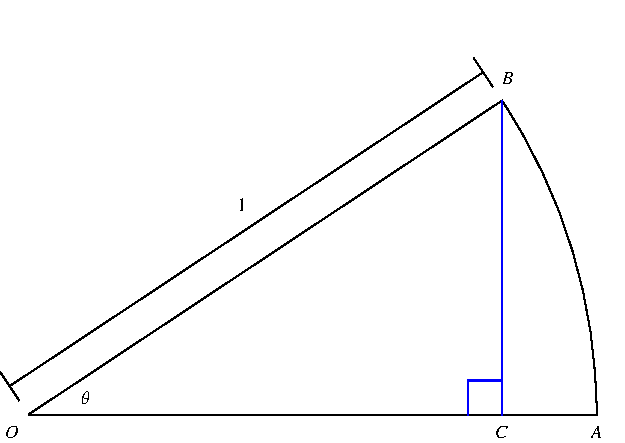
\includegraphics[width=4.5cm]{derivatives-trig/pictures/03-04-proofa.pdf}%
%}%
%\only<handout:0| 4-9>{%
%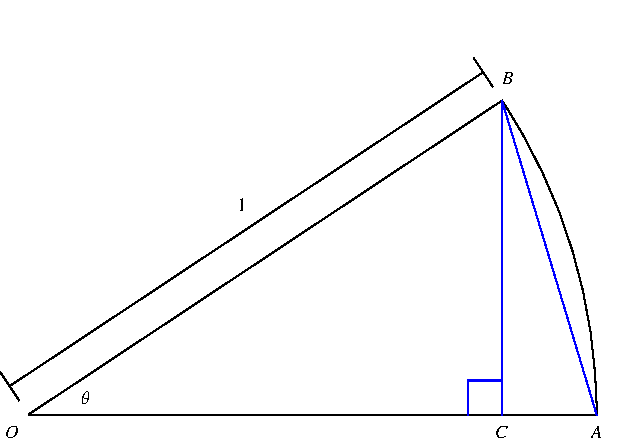
\includegraphics[width=4.5cm]{derivatives-trig/pictures/03-04-proofb.pdf}%
%}%
%\only<handout:0| 10>{%
%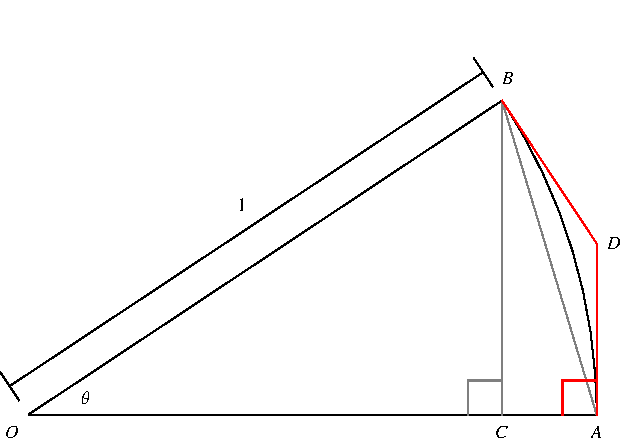
\includegraphics[width=4.5cm]{derivatives-trig/pictures/03-04-proofc.pdf}%
%}%
%\only<11->{%
%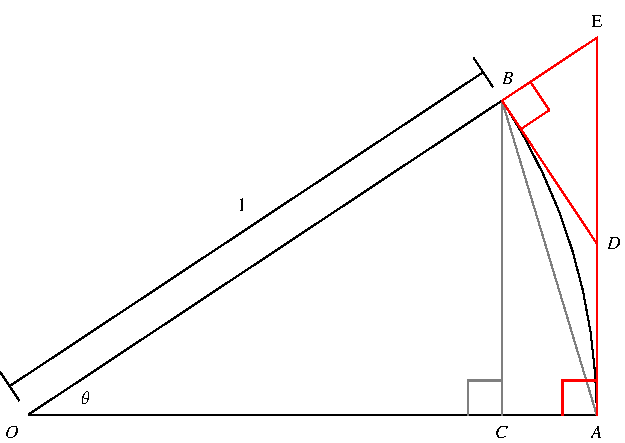
\includegraphics[width=4.5cm]{derivatives-trig/pictures/03-04-proofd.pdf}%
%}%

\end{columns}
\[
\uncover<2->{%
\alert<handout:0| 2-5>{%
\sin \theta = \uncover<3->{\frac{|BC|}{|OB|}=|BC|} %
}%
}%
\uncover<4->{%
\alertNoH{4-5}{< |AB|}%
}%
\uncover<5->{%
 \alertNoH{5}{<} \alert<handout:0| 5-7>{\text{arc} AB \uncover<6->{ = } \uncover<7->{\theta}}%
}%
\]
\uncover<8->{%
Therefore $\alert<handout:0| 18>{\frac{\sin \theta}{\theta} < 1}$.%
}%
\abovedisplayskip=0pt
\belowdisplayskip=0pt
\begin{align*}
\uncover<9->{%
\theta = \text{arc} AB %
}%
& \uncover<10->{ < }  %
\uncover<10->{%
\alertNoH{10}{|AD|} + \alert<handout:0| 10,11>{|DB|}%
}  \uncover<11->{ < }  \uncover<11->{%
|AD| + \alert<handout:0| 11>{|DE|}%
}\\%
& \uncover<12->{ = }  %
\uncover<12->{%
\alertNoH{12-14}{
|AE|%
}
}%
\uncover<13->{%
 = |OA| \tan \theta
}  \uncover<14->{ = }  \uncover<14->{%
\alertNoH{14}{
\tan \theta%
}
}%
\end{align*}
\uncover<15->{%
Therefore $\theta < \tan \theta = \frac{\sin \theta}{\cos \theta}$, so $\alert<handout:0| 17>{\cos \theta < \frac{\sin \theta}{\theta}}$.
}%

\uncover<16->{%
\abovedisplayskip=0pt
\belowdisplayskip=0pt
\[
\alert<handout:0| 17>{\cos \theta < }%
\alert<handout:0| 17-18>{\frac{\sin \theta}{\theta}}%
\alert<handout:0| 18>{ < 1}%
\]
\uncover<19->{%
\alert<handout:0| 20-21>{$\lim_{\theta\rightarrow 0}\cos \theta = \uncover<21->{1}$} and \alert<handout:0| 22-23>{$\lim_{\theta\rightarrow 0} 1 = \uncover<23->{1}$}\uncover<23->{, so by the Squeeze Theorem $\lim_{\theta \rightarrow 0^+}\frac{\sin \theta}{\theta} = 1$.}  \uncover<24->{$\frac{\sin \theta}{\theta}$ is even, so the left limit is also 1.}
}%
}%
\end{frame}

\begin{frame}
\abovedisplayskip=0pt
\belowdisplayskip=0pt
\abovedisplayshortskip=0pt
\belowdisplayshortskip=0pt
\begin{align*}
\text{Let}\quad f(x) & = \sin x. \\
\text{Then}\quad f'(x) & =  %
\uncover<1->{%
\alert<handout:0| 2-3>{\lim_{h\rightarrow 0} \sin x}\cdot \alert<handout:0| 4-5>{\lim_{h\rightarrow 0} \frac{\cos h - 1}{h}} + \alert<handout:0| 6-7>{\lim_{h\rightarrow 0}\cos x}\cdot \alert<handout:0| 8-9>{\lim_{h\rightarrow 0}  \frac{\sin h}{h}}  %
}\\%
& \uncover<2->{ = }  %
\uncover<2->{%
\uncover<3->{\alert<handout:0| 3>{ \sin x}} \uncover<5->{\cdot\alert<handout:0| 5,10>{\lim_{h\rightarrow 0} \frac{\cos h - 1}{h}}} \uncover<7->{+ \alert<handout:0| 7>{\cos x}} \uncover<9->{\cdot\alert<handout:0| 9>{1}}  %
}%
\uncover<10->{%
\intertext{We need to find}%
}%
\uncover<10->{%
\lim_{h\rightarrow 0}\frac{\cos h - 1}{h}%
}%
& \uncover<11->{ = }  %
\uncover<11->{%
\lim_{h\rightarrow 0}\left( \frac{\cos h - 1}{h} \cdot \frac{\cos h + 1}{\cos h + 1}\right)%
}  \uncover<12->{ = } \uncover<12->{%
\lim_{h\rightarrow 0} \frac{\alert<handout:0| 13>{\cos^2 h - 1}}{h(\cos  h + 1)}%
}\\%
& \uncover<13->{ = }  %
\uncover<13->{%
\lim_{h\rightarrow 0} \frac{\alert<handout:0| 13>{-\sin^2 h}}{h(\cos  h + 1)}%
}  \uncover<14->{ = } \uncover<14->{%
-\lim_{h\rightarrow 0} \left( \frac{\sin h}{h}\cdot \frac{\sin h}{\cos h + 1}\right)%
}\\%
& \uncover<15->{ = }  %
\uncover<15->{%
-\alert<handout:0| 16>{\lim_{h\rightarrow 0}  \frac{\sin h}{h}}\cdot\lim_{h\rightarrow 0} \frac{\sin h}{\cos h + 1}%
}  \uncover<16->{ = } \uncover<16->{%
-\alert<handout:0| 16>{1}\cdot \left( \frac{0}{1+1}\right)%
}  \uncover<17->{ = } \uncover<17->{%
0
}%
\end{align*}

\uncover<18->{%
\begin{theorem}[The Derivative of $\sin x$]
\[
\frac{\diff}{\diff x} \sin x = \cos x
\]
\end{theorem}
}%
\end{frame}
% end module derivative-sine
